
\usepackage{fancyhdr}
\usepackage{lastpage}
\usepackage[utf8]{inputenc}

% Minted for syntax highliting
\usepackage{minted}
\usemintedstyle{tango}

% 
\usepackage[T1]{fontenc}
\usepackage{lmodern}

\usepackage{calc}
\usepackage{bytefield}

\usepackage{listings}
\usepackage{amsmath}

\usepackage{tikz}
\usetikzlibrary{automata,arrows,topaths,calc,positioning}
 
\usepackage{syntax}
\grammarindent=2cm


% Headers/footers styling
\pagestyle{fancy}
\fancyhf{}
\renewcommand{\headrulewidth}{0pt}

% Footer
\lfoot{ID1019}
\cfoot{KTH}
\rfoot{\thepage \hspace{1pt} / \pageref{LastPage}}

%\newcommand{\defaultpagestyle}{\thispagestyle{plain}}
\newcommand{\defaultpagestyle}{\thispagestyle{fancy}}



\title[ID1019 Complexity]{Complexity}


\author{Johan Montelius}
\institute{KTH}
\date{\semester}

\begin{document}

\begin{frame}
\titlepage
\end{frame}

\begin{frame}[fragile]{run-time complexity of sum}

Calculating the sum of all elements in a list:

\pause\vspace{20pt}

\begin{columns}
   \begin{column}{.5\linewidth}
     \begin{block}{sum/1}
       \begin{verbatim}
def sum([]) do 0 end
def sum([h|t]) do 
   s = sum(t)
   h + s
end
       \end{verbatim}
      \end{block}
    \end{column}
\pause
    \begin{column}{.5\linewidth}
     \begin{block}{sum/2}
       \begin{verbatim}
def sum([], s) do s end
def sum([h|t], s) do
   s1 = h+s 
   sum(t, s1)
end
       \end{verbatim}
      \end{block}
    \end{column}
  \end{columns}

\pause\vspace{20pt}
What are the run-time complexities of sum/1 and sum/2?

\end{frame}

\begin{frame}[fragile]{run-time complexity of foo}


\pause\vspace{20pt}
\begin{columns}
   \begin{column}{.5\linewidth}
     \begin{block}{foo/1}
       \begin{verbatim}
def foo([]) do [] end
def foo([h|t]) do
   z = foo(t)
   bar(z, h)
end
       \end{verbatim}
      \end{block}
    \end{column}
\pause
    \begin{column}{.5\linewidth}
     \begin{block}{foo/2}
       \begin{verbatim}
def foo([], y) do y  end
def foo([h|t], y) do
   z = zot(h, y)
   foo(t, z)
end
       \end{verbatim}
      \end{block}
    \end{column}
  \end{columns}

\pause\vspace{20pt}
What are the run-time complexities of foo/1 and foo/2?

\end{frame}


\begin{frame}[fragile]{run-time complexity of reverse}

\pause\vspace{20pt}
\begin{columns}
   \begin{column}{.5\linewidth}
     \begin{block}{nreverse/1}
       \begin{verbatim}
def nreverse([]) do [] end
def nreverse([h|t]) do 
   z = nreverse(t)
   append(z, [h])
end
       \end{verbatim}
      \end{block}
    \end{column}
\pause
    \begin{column}{.5\linewidth}
     \begin{block}{reverse/2}
       \begin{verbatim}
def reverse([], y) do y end
def reverse([h|t], y) do 
   z = [h | y]
   reverse(t, z)
end
       \end{verbatim}
      \end{block}
    \end{column}
  \end{columns}

\pause\vspace{20pt}
What are the run-time complexities of nreverse/1 and reverse/2?

\end{frame}

\begin{frame}[fragile]{the recurence relation}

\begin{columns}
   \begin{column}{.4\linewidth}
     \begin{block}{nreverse/1}
       \begin{verbatim}
def nreverse([]) do [] end
def nreverse([h|t]) do 
   z = nreverse(t)
   append(z, [h])
end
       \end{verbatim}
      \end{block}
    \end{column}
\pause
    \begin{column}{.6\linewidth}
      Assume that {\tt append/2} takes $kn$ ms to execute, where $k$
      is some constant time and $n$ is the length of the list. \pause

      \vspace{5pt} Describe the time $T_n$ it takes to execute {\tt
        nreverse/1} of a list of length $n$: \pause

      \vspace{5pt}      
      $T_0 = a {\rm \ ms}$ \pause
      
      $T_n = T_{n-1} + k(n-1) + b {\rm \ ms}$ \pause
    \end{column}
  \end{columns}
  
\end{frame}


\begin{frame}[fragile]{the recurence relation}

\begin{equation}  
  \begin{split}
T_n & = T_{n-1} + k(n-1) + b \\ 
    & \onslide<2->{ = T_{n-2} + k(n-2) + k(n-1) + 2b }\\
    & \onslide<3->{= T_{n-3} + k(n-3) + k(n-2) + k(n-1) + 3b }\\ 
    & \onslide<4->{:} \\
    & \onslide<4->{= T_{n-n} + k(n-n) + ...... k(n-1)  + nb }\\
    & \onslide<5->{= a + 0 + k + 2k + 3k ...... (n-1)k  + nb  }\\ 
    & \onslide<6->{= n\frac{(n-1)}{2}k + nb + a }\\ 
    & \onslide<7->{= (\frac{k}{2})n^2 - \frac{k}{2}n+ bn + a }\\
    & \onslide<8->{= (\frac{k}{2})n^2 + (b - \frac{k}{2})n+  a }\\    
  \end{split} 
\end{equation}

\end{frame}

\begin{frame}[fragile]{the big-O notation}

  We know:

  \vspace{10pt}\pause

  $$T_n  = (\frac{k}{2})n^2 + (b -\frac{k}{2})n+ a $$

  \vspace{20pt}\pause

  $$T_n \in O(n^2)$$
  
\end{frame}

\begin{frame}{Ordo calculations}

  Do ordo calculations in your head without specifying the full $T_n$
  relation. \pause

  \vspace{10pt}If we know that {\tt append/2} is in $O(n)$ then: \pause
  
  $$ T_n \in n * O(n) + bn + a$$ 

  \vspace{10pt}Which means that:

  $$ T_n \in O(n^2)$$

\end{frame}



\begin{frame}[fragile]{run-time complexity of reverse/1}

\begin{columns}
  \begin{column}{.5\linewidth}
     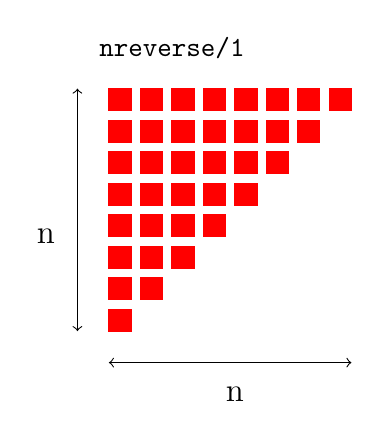
\begin{tikzpicture}[scale=0.4]
        \node at (2,10) {{\tt nreverse/1}};
        \pause
        \filldraw [red] (0,8) rectangle +(0.7,0.7); 
        \filldraw [red] (1,8) rectangle +(0.7,0.7); 
        \filldraw [red] (2,8) rectangle +(0.7,0.7); 
        \filldraw [red] (3,8) rectangle +(0.7,0.7); 
        \filldraw [red] (4,8) rectangle +(0.7,0.7); 
        \filldraw [red] (5,8) rectangle +(0.7,0.7); 
        \filldraw [red] (6,8) rectangle +(0.7,0.7); 
        \filldraw [red] (7,8) rectangle +(0.7,0.7); 
        \pause
        \filldraw [red] (0,7) rectangle +(0.7,0.7); 
        \filldraw [red] (1,7) rectangle +(0.7,0.7); 
        \filldraw [red] (2,7) rectangle +(0.7,0.7); 
        \filldraw [red] (3,7) rectangle +(0.7,0.7); 
        \filldraw [red] (4,7) rectangle +(0.7,0.7); 
        \filldraw [red] (5,7) rectangle +(0.7,0.7); 
        \filldraw [red] (6,7) rectangle +(0.7,0.7); 
        \pause
        \filldraw [red] (0,6) rectangle +(0.7,0.7); 
        \filldraw [red] (1,6) rectangle +(0.7,0.7); 
        \filldraw [red] (2,6) rectangle +(0.7,0.7); 
        \filldraw [red] (3,6) rectangle +(0.7,0.7); 
        \filldraw [red] (4,6) rectangle +(0.7,0.7); 
        \filldraw [red] (5,6) rectangle +(0.7,0.7); 
        \pause
        \filldraw [red] (0,5) rectangle +(0.7,0.7); 
        \filldraw [red] (1,5) rectangle +(0.7,0.7); 
        \filldraw [red] (2,5) rectangle +(0.7,0.7); 
        \filldraw [red] (3,5) rectangle +(0.7,0.7); 
        \filldraw [red] (4,5) rectangle +(0.7,0.7); 
        \pause
        \filldraw [red] (0,4) rectangle +(0.7,0.7); 
        \filldraw [red] (1,4) rectangle +(0.7,0.7); 
        \filldraw [red] (2,4) rectangle +(0.7,0.7); 
        \filldraw [red] (3,4) rectangle +(0.7,0.7); 
        \pause
        \filldraw [red] (0,3) rectangle +(0.7,0.7); 
        \filldraw [red] (1,3) rectangle +(0.7,0.7); 
        \filldraw [red] (2,3) rectangle +(0.7,0.7); 
        \pause
        \filldraw [red] (0,2) rectangle +(0.7,0.7); 
        \filldraw [red] (1,2) rectangle +(0.7,0.7); 
        \pause
        \filldraw [red] (0,1) rectangle +(0.7,0.7);



        
        
        \pause


        
        \draw [<->] (-1,1) -- (-1,8.7); 
        \pause
        \node at (-2, 4) {{\large n}};
        \pause
        \draw [<->] (0,0) -- (7.7,0);         
        \pause
        \node at (4, -1) {{\large n}};

     \end{tikzpicture}
   \end{column}
   
   \begin{column}{.5\linewidth}
     \begin{block}{nreverse/1}
       \begin{verbatim}
def nreverse([]) do  end
def nreverse([h|t]) do 
   z = nreverse(t)
   append(z, [h])
end
       \end{verbatim}
     \end{block}
   \end{column}
 \end{columns}

\end{frame}


\begin{frame}[fragile]{run-time complexity of reverse/2}

  \begin{columns}
    \begin{column}{.5\linewidth}
      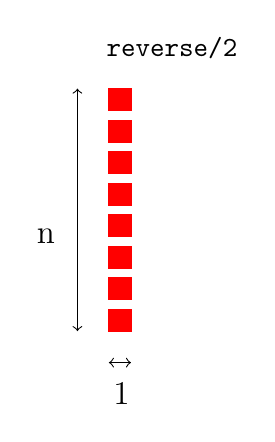
\begin{tikzpicture}[scale=0.4]
        \node at (2,10) {{\tt reverse/2}};
        \filldraw [red] (0,8) rectangle +(0.7,0.7); 
        \filldraw [red] (0,7) rectangle +(0.7,0.7); 
        \filldraw [red] (0,6) rectangle +(0.7,0.7); 
        \filldraw [red] (0,5) rectangle +(0.7,0.7); 
        \filldraw [red] (0,4) rectangle +(0.7,0.7); 
        \filldraw [red] (0,3) rectangle +(0.7,0.7); 
        \filldraw [red] (0,2) rectangle +(0.7,0.7); 
        \filldraw [red] (0,1) rectangle +(0.7,0.7); 
        \pause
        \draw [<->] (-1,1) -- (-1,8.7); 
        \pause
        \node at (-2, 4) {{\large n}};
        \pause
        \draw [<->] (0,0) -- (0.7,0);         
        \pause
        \node at (0.4, -1) {{\large 1}};
      \end{tikzpicture}

    \end{column}


    \begin{column}{.5\linewidth}
      \begin{block}{reverse/2}
        \begin{verbatim}
def reverse([], y) do y end
def reverse([h|t], y) do 
   z = [h | y]
   reverse(t, z)
end
       \end{verbatim}
      \end{block}
    \end{column}
  \end{columns}

\end{frame}




\begin{frame}[fragile]{complexity of quick-sort}

\begin{columns}
   \begin{column}{.5\linewidth}
    \begin{verbatim}
def qsort([]) do [] end
def qsort([h]) do [h] end
def qsort(all) do 
   {low, high} = partition(all)
   lowS = qsort(low)
   highS = qsort(high)
   append(lowS, highS)
end
    \end{verbatim}
   \end{column}
   \begin{column}{.5\linewidth}
    \begin{itemize}
      \pause \item What is done in each iteration?
      \pause \item How many iterations do we have?       
    \end{itemize}
   \end{column}
\end{columns}


\end{frame}

\begin{frame}{the recurence relation}

\begin{equation}  
\begin{split}
    T_1 & = a \\
\\
T_n & = 2 \times T_{n/2} + nc \\ 
    &\onslide<2->{ = 2 \times ( 2 \times T_{n/4} + (n/2)c ) + nc }\\
    &\onslide<3->{ = 4 \times T_{n/4} + 2 \times nc}\\
    &\onslide<3->{ = 8 \times T_{n/8} + 3 \times nc}\\
    &\onslide<3->{ : }\\
    &\onslide<4->{ = 2^k \times T_1 + k \times nc }\\
    &\onslide<5->{ = 2^{lg(n)} \times a  + lg(n) \times nc }\\
    &\onslide<6->{ = n \times a + lg(n)n \times c}\\
  \end{split}
\end{equation}

\end{frame}


\begin{frame}{complexity of quick-sort}
     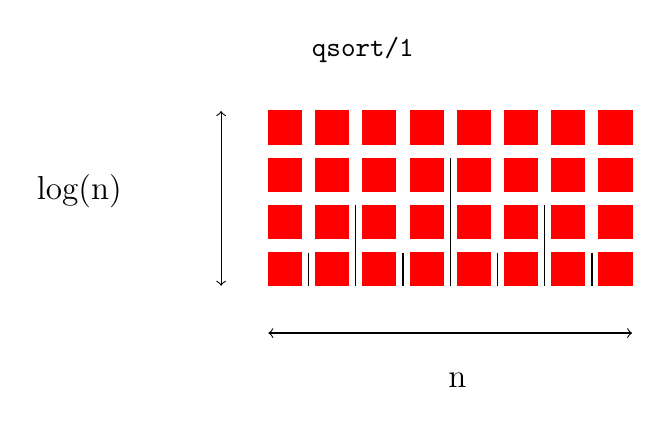
\begin{tikzpicture}[scale=0.6]

        \node at (2,10) {{\tt qsort/1}};
        \filldraw [red] (0,8) rectangle +(0.7,0.7); 
        \filldraw [red] (1,8) rectangle +(0.7,0.7); 
        \filldraw [red] (2,8) rectangle +(0.7,0.7); 
        \filldraw [red] (3,8) rectangle +(0.7,0.7); 
        \filldraw [red] (4,8) rectangle +(0.7,0.7); 
        \filldraw [red] (5,8) rectangle +(0.7,0.7); 
        \filldraw [red] (6,8) rectangle +(0.7,0.7); 
        \filldraw [red] (7,8) rectangle +(0.7,0.7); 
        \pause
        \draw [black] (3.85, 7.7) -- (3.85, 5);

        \filldraw [red] (0,7) rectangle +(0.7,0.7); 
        \filldraw [red] (1,7) rectangle +(0.7,0.7); 
        \filldraw [red] (2,7) rectangle +(0.7,0.7); 
        \filldraw [red] (3,7) rectangle +(0.7,0.7); 
        \pause
        \filldraw [red] (4,7) rectangle +(0.7,0.7); 
        \filldraw [red] (5,7) rectangle +(0.7,0.7); 
        \filldraw [red] (6,7) rectangle +(0.7,0.7); 
        \filldraw [red] (7,7) rectangle +(0.7,0.7); 

        \pause
        \draw [black] (1.85, 6.7) -- (1.85, 5);
        \draw [black] (5.85, 6.7) -- (5.85, 5);

        \pause
        \filldraw [red] (0,6) rectangle +(0.7,0.7); 
        \filldraw [red] (1,6) rectangle +(0.7,0.7); 
        \pause
        \filldraw [red] (2,6) rectangle +(0.7,0.7); 
        \filldraw [red] (3,6) rectangle +(0.7,0.7); 
        \pause
        \filldraw [red] (4,6) rectangle +(0.7,0.7); 
        \filldraw [red] (5,6) rectangle +(0.7,0.7); 
        \pause
        \filldraw [red] (6,6) rectangle +(0.7,0.7); 
        \filldraw [red] (7,6) rectangle +(0.7,0.7); 

        \pause
        \draw [black] (0.85, 5.7) -- (0.85, 5);
        \draw [black] (2.85, 5.7) -- (2.85, 5);
        \draw [black] (4.85, 5.7) -- (4.85, 5);
        \draw [black] (6.85, 5.7) -- (6.85, 5);

        \pause
        \filldraw [red] (0,5) rectangle +(0.7,0.7); 
        \pause
        \filldraw [red] (1,5) rectangle +(0.7,0.7); 
        \pause
        \filldraw [red] (2,5) rectangle +(0.7,0.7); 
        \pause
        \filldraw [red] (3,5) rectangle +(0.7,0.7); 
        \pause
        \filldraw [red] (4,5) rectangle +(0.7,0.7); 
        \pause
        \filldraw [red] (5,5) rectangle +(0.7,0.7); 
        \pause
        \filldraw [red] (6,5) rectangle +(0.7,0.7); 
        \pause
        \filldraw [red] (7,5) rectangle +(0.7,0.7); 


        \pause
        \draw [<->] (-1,5) -- (-1,8.7); 
        \pause
        \node at (-4, 7) {{\large log(n)}};
        \pause
        \draw [<->] (0,4) -- (7.7,4);         
        \pause
        \node at (4, 3) {{\large n}};

     \end{tikzpicture}

\end{frame}

\begin{frame}{qsort worst case}

What if we run qsort on a already ordered list?

\end{frame}


\begin{frame}[fragile]{complexity of merge-sort}

\begin{columns}
   \begin{column}{.5\linewidth}
    \begin{verbatim}
def msort([]) do [] end
def msort(l) do
   {a, b} = split(l)
   as = msort(a)
   bs = msort(b)
   merge(as, bs)
end
   \end{verbatim}
   \end{column}
   \begin{column}{.5\linewidth}
    \begin{itemize}
      \pause \item What is done in each iteration?
      \pause \item How many iterations do we have?       
      \pause \item What is the run-time complexity?       
      \pause \item Which is best qsort or msort?       
    \end{itemize}
   \end{column}
\end{columns}

\end{frame}

\begin{frame}[fragile]{complexity of fibonacci}

\begin{columns}
   \begin{column}{.5\linewidth}
    \begin{verbatim}
def fib(0) do 0 end
def fib(1) do 1 end
def fib(n) do 
   fib(n-1) + fib(n-2)
end
    \end{verbatim}
   \end{column}
   \begin{column}{.5\linewidth}
    \begin{itemize}
      \pause \item What is done in each iteration?
      \pause \item How many iterations do we have?       
    \end{itemize}
   \end{column}
\end{columns}

\end{frame}

\begin{frame}{the recurence relation}

  Let's cheat a bit to make it simpler:

  \vspace{5pt}\pause

    \begin{equation}  
  \begin{split}
    T_0 & = a \\
    \\
T_n & = 2 \times T_{n-1} + c \\
    &\onslide<2->{ = 2 \times ( 2 \times T_{n-2} + c ) + c }\\
    &\onslide<3->{ = 4 \times T_{n-2} + 3 \times c }\\
    &\onslide<4->{ = 8 \times T_{n-3} + 7 \times c}\\
    &\onslide<4->{ : }\\
    &\onslide<5->{ = 2^n \times T_0 +  (2^n -1) \times c }\\
    &\onslide<6->{ = 2^n \times a +  2^n \times c  - c}\\
  \end{split}
\end{equation}

\vspace{5pt}\pause
\pause  {\em The more precise answer is $O(1.6^n)$}


\end{frame}


\begin{frame}{complexity of fibonacci}
     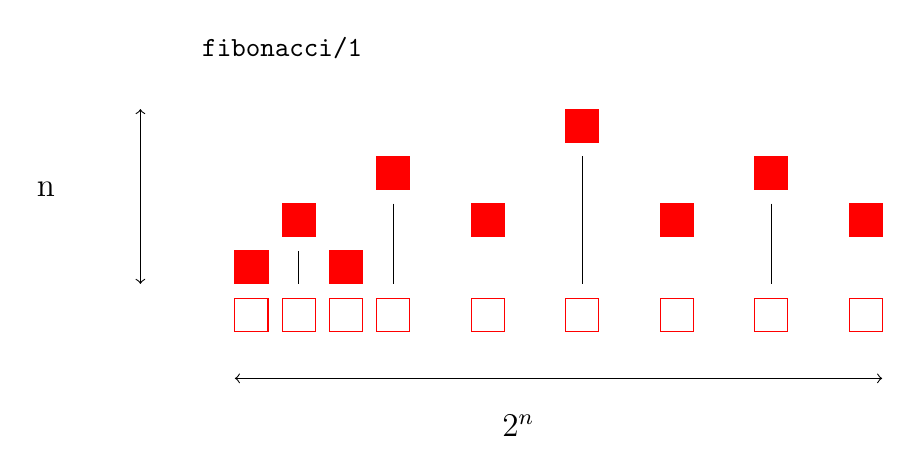
\begin{tikzpicture}[scale=0.6]

        \node at (2,10) {{\tt fibonacci/1}};
        \filldraw [red] (8,8) rectangle +(0.7,0.7);  % fib(4)
        \pause
        \draw [black] (8.35, 7.7) -- (8.35, 5);

        \pause
        \filldraw [red] (4,7) rectangle +(0.7,0.7);  % fib(3)
        \filldraw [red] (12,7) rectangle +(0.7,0.7); % fib(2)
        \pause
        \draw [black] (4.35, 6.7) -- (4.35, 5);
        \draw [black] (12.35, 6.7) -- (12.35, 5);


        \pause
        \filldraw [red] (2,6) rectangle +(0.7,0.7);  % fib(2)
        \filldraw [red] (6,6) rectangle +(0.7,0.7); % fib(1)

        \filldraw [red] (10,6) rectangle +(0.7,0.7);  % fib(1)
        \filldraw [red] (14,6) rectangle +(0.7,0.7); % fib(0)

        \draw [black] (2.35, 5.7) -- (2.35, 5);

        \pause

        \filldraw [red] (1,5) rectangle +(0.7,0.7);  % fib(1)
        \filldraw [red] (3,5) rectangle +(0.7,0.7);  % fib(0)

        \pause
        \draw [red] (8,4) rectangle +(0.7,0.7);  % fib(4)
        \draw [red] (4,4) rectangle +(0.7,0.7);  % fib(3)
        \draw [red] (12,4) rectangle +(0.7,0.7); % fib(2)

        \draw [red] (2,4) rectangle +(0.7,0.7);  % fib(2)
        \draw [red] (6,4) rectangle +(0.7,0.7); % fib(1)

        \draw [red] (10,4) rectangle +(0.7,0.7);  % fib(1)
        \draw [red] (14,4) rectangle +(0.7,0.7); % fib(0)
        \draw [red] (1,4) rectangle +(0.7,0.7);  % fib(1)
        \draw [red] (3,4) rectangle +(0.7,0.7);  % fib(0)

        \pause
        \draw [<->] (-1,5) -- (-1,8.7); 
        \pause
        \node at (-3, 7) {{\large n}};
        \pause
        \draw [<->] (1,3) -- (14.7,3);         
        \pause
        \node at (7, 2) {{\large $2^n$}};
     \end{tikzpicture}

\pause  The smarter implementation is $O(n)$

\pause  {\em ... an even smart solution is $O(log(n))$}

\end{frame}

\begin{frame}{The big question}

What is the difference between a smart programmer and a not so smart programmer?

\vspace{60pt}
\pause \centerline{3 billion years?}

\end{frame}

\begin{frame}[fragile]{operations on trees}

  Let's represent trees as:
  \vspace{10pt}
  
\begin{verbatim}
 :nil
{:node, key, value, left, right}
\end{verbatim}

\pause \vspace{20pt}
\begin{itemize}
\item new: create a empty tree
\item insert: add an element to the three
\item lookup: search for an element 
\item modify: modify an element
\end{itemize}

\end{frame}

\begin{frame}{why trees?}

Why use trees, why not use lists?

\end{frame}

\begin{frame}{benchmark tree operations}
 Operations on a tree.
 \begin{figure}
  \centering
  \includegraphics[height=140pt]{tree.png}
  \caption{Execution time in ms of 100.000 calls}
 \end{figure}

\end{frame}

\begin{frame}{why trees?}

\pause \vspace{40pt}
Why use trees, why not use tuples?

\end{frame}

\begin{frame}[fragile]{tuples as a key value store}

\begin{verbatim}
def new([a,b,c]) do {a,b,c} end
\end{verbatim}
\pause
\begin{verbatim}
def lookup({a,_,_}, 1) do a end
def lookup({_, b,_}, 2) do b end
  :
\end{verbatim}
\pause
\begin{verbatim}
def modify({_,b,c}, 1, v) do {v, b, c} end
def modify({a,_,c}, 2, v) do {a, v, c} end
  :

\end{verbatim}

\end{frame}

\begin{frame}[fragile]{tuples using builtin functions}

  
\begin{verbatim}
def new(list) do List.to_tuple(list) end
\end{verbatim}
\pause
\begin{verbatim}
def lookup(tuple, k) do elem(tuple, k) end  
def modify(tuple, k, v) do put_elem(tuple, k, v) end
\end{verbatim}
\pause

\pause{\em The functions put_elem/3 will create a copy of the original tuple!}

\end{frame}


\begin{frame}{benchmark tuple operations}
 Operations on a tuple.
 \begin{figure}
  \centering
  \includegraphics[height=140pt]{table.png}
  \caption{Execution time in ms of 100.000 calls}
 \end{figure}

\end{frame}



\begin{frame}{compare tuples and trees}
 Tuple vs tree.
 \begin{figure}
  \centering
  \includegraphics[height=140pt]{comp.png}
  \caption{Modify operations, execution time in ms of 100.000 calls}
 \end{figure}

\end{frame}

\begin{frame}{root of all evil}

\begin{quote}
Programmers waste enormous amounts of time thinking about, or
worrying about, the speed of noncritical parts of their programs, and
these attempts at efficiency actually have a strong negative impact
when debugging and maintenance are considered. We should forget about
small efficiencies, say about 97 percent of the time: premature
optimization is the root of all evil. Yet we should not pass up our
opportunities in that critical 3 percent.
\end{quote}

 {\em Donald Knuth}


\end {frame}

\begin{frame}{code vs time}

     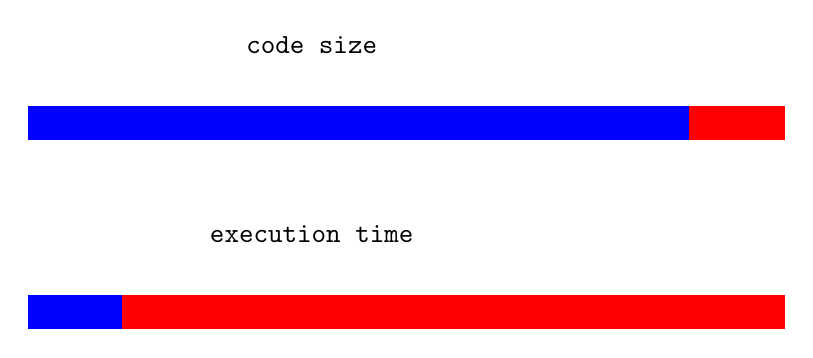
\begin{tikzpicture}[scale=0.6]

        \node at (8,10) {{\tt code size}};
        \filldraw [blue] (2,8) rectangle +(14,0.7);  % 
        \filldraw [red] (16,8) rectangle +(2,0.7);  % 
        \pause

        \node at (8,6) {{\tt execution time}};
        \filldraw [blue] (2,4) rectangle +(2,0.7);  % 
        \filldraw [red] (4,4) rectangle +(14,0.7);  % 
        \pause
   \end{tikzpicture}
\end{frame}

\begin{frame}{programming rules}

\begin{itemize}
\pause
\item understand the problem before starting coding
\pause
\item write well structured code that is easy to understand
\pause
\item use abstractions to separate functionality from implementation
\pause
\item think about complexity
\pause
\item benchmark your program 
\pause
\item if needed, optimize
\end{itemize}

\end{frame}


\end{document}


